\documentclass[11pt,a4paper]{article}

\usepackage[margin=1in]{geometry}
\usepackage{graphicx}
\usepackage{booktabs}
\usepackage{amsmath,amssymb}
\usepackage{hyperref}
\usepackage{xcolor}
\usepackage{caption}
\usepackage{subcaption}
\usepackage{float}
\usepackage{multirow}
\usepackage{appendix}

\hypersetup{colorlinks=true,linkcolor=blue!60!black,citecolor=blue!60!black,urlcolor=blue!60!black}

\title{Fixed-Compute Scaling of AR and Diffusion Language Models\\[4pt]
\large An IsoFLOP Study on TinyShakespeare}
\author{Chang-Han}
\date{March 2026}

\begin{document}
\maketitle

\begin{abstract}
We study how a fixed training budget should be split between model size and training duration for small language models.
Using a shared transformer backbone, we compare five training objectives: autoregressive (AR), Remasked, MDLM, Edit-one-pass, and Edit-two-pass.
On TinyShakespeare (${\sim}1$M characters), we run 91 IsoFLOP experiments across four budgets and six model sizes.

Two patterns dominate.
First, every family exhibits the expected U-shaped validation-loss curve at fixed compute, but the minima move differently.
AR leaves the 0.3M regime by the second budget, while Remasked and MDLM stay there until the third.
At budget C2, for example, AR prefers 1M parameters trained for 1015 steps, whereas Remasked and MDLM prefer 0.3M trained for 2948 steps.
Second, the overfitting gap explains much of this difference.
At each family's optimum, AR's validation-minus-training gap grows from 0.195 to 0.479 across budgets, while the diffusion families stay at or below 0.175 and are slightly underfit at the smallest budget.

The simplest interpretation is that masking noise acts as built-in regularization: diffusion models can productively spend extra FLOPs on more updates, while AR reaches the memorization regime sooner.
This is a toy-scale study, not a verdict on overall model quality.
Cross-family validation cross-entropy is not directly comparable, and the highest budget is partially shaped by a 10k-step cap.
But as a controlled scaling diagnostic, the contrast is clear and motivates larger-scale follow-up.
\end{abstract}

%% ===================================================================
\section{Introduction}
\label{sec:intro}

Chinchilla-style scaling laws ask a concrete question: under a fixed compute budget, how should training be divided between model size and token budget?
That question is usually posed within a single model family, almost always autoregressive.
Here we ask whether the answer changes when the training objective changes.

This is a useful place to compare AR and diffusion language models.
The two paradigms do not merely decode differently; they may spend compute differently during training.
If denoising objectives provide implicit regularization, then the compute-optimal tradeoff between parameters and updates may shift in a systematic way.

We study this in a deliberately small and controlled setting.
TinyShakespeare makes failure modes easy to see: large AR models can memorize it quickly, while undertrained models are also easy to identify.
That makes the dataset a reasonable diagnostic environment for IsoFLOP behavior, even if it is far too small for broad performance claims.

\paragraph{What this paper contributes.}
\begin{enumerate}
    \item A controlled IsoFLOP comparison across five language-model training objectives with matched backbones.
    \item Evidence that AR and diffusion families allocate extra compute differently in the small-data regime.
    \item A simple mechanistic hypothesis: masking noise suppresses overfitting enough that diffusion models can profitably train longer before needing to scale up.
\end{enumerate}

%% ===================================================================
\section{Setup}
\label{sec:setup}

\subsection{Five Families, One Backbone}

All five models use the same character-level transformer backbone: RoPE with QK-norm, $n_\text{head}=4$, ReGLU MLP, RMSNorm, and no bias terms.
The only changes are the attention mask and the training objective:

\begin{enumerate}
    \item \textbf{AR.} Standard next-token prediction with causal attention.
    \item \textbf{Remasked.} Predict all tokens, then remask low-confidence positions according to the noise schedule.
    \item \textbf{MDLM.} Progressive unmasking: once a token is revealed, it stays revealed.
    \item \textbf{Edit-one-pass.} Denoise both masked positions and corrupted visible tokens.
    \item \textbf{Edit-two-pass.} A denoising pass followed by a correction pass, at roughly $2\times$ the FLOP cost per training step.
\end{enumerate}

We test six model sizes (0.1M to 3.2M parameters; Table~\ref{tab:sizes}) and four FLOP budgets ($6\!\times\!10^{13}$ to $2\!\times\!10^{15}$).
Learning rate and batch size come from a small sweep (Appendix~\ref{app:sweep}).
AR uses dropout\,=\,0.2; the diffusion families use dropout\,=\,0.1 because additional dropout consistently hurt them (Appendix~\ref{app:dropout}).

\begin{table}[H]
\centering
\caption{Model size configurations. All use $n_\text{head}=4$.}
\label{tab:sizes}
\begin{tabular}{lcccr}
\toprule
Label & $n_\text{embd}$ & $n_\text{layer}$ & head\_dim & Parameters \\
\midrule
0.1M & 64 & 2 & 16 & 107K \\
0.3M & 96 & 3 & 24 & 345K \\
0.5M & 120 & 3 & 30 & 535K \\
1M & 128 & 5 & 32 & 1.00M \\
2M & 200 & 4 & 50 & 1.95M \\
3M & 256 & 4 & 64 & 3.18M \\
\bottomrule
\end{tabular}
\end{table}

\subsection{IsoFLOP Protocol}

Training FLOPs are approximated as $6 \times N \times T_\text{tokens}$ for standard models and $12 \times N \times T_\text{tokens}$ for Edit-two-pass.
At each budget we train every feasible $(\text{family}, \text{size})$ pair for the number of steps that consumes that budget, then record the final train and validation cross-entropy.
Within each family, the compute-optimal size is the one with the lowest validation CE.

\begin{table}[H]
\centering
\caption{IsoFLOP budget matrix. Entries show training steps; --- indicates infeasible (outside step bounds $[150, 10000]$). Budget C2 achieves full coverage: all 5 families $\times$ 6 sizes.}
\label{tab:isoflop-matrix}
\begin{tabular}{lrrrrrr}
\toprule
Budget & 0.1M & 0.3M & 0.5M & 1M & 2M & 3M \\
\midrule
C1 ($6\!\times\!10^{13}$)  & 2852 & 884 & 570 & 304 & 156 & --- \\
C2 ($2\!\times\!10^{14}$)  & 9507 & 2948 & 1901 & 1015 & 521 & 319 \\
C3 ($6\!\times\!10^{14}$)  & --- & 8845 & 5703 & 3045 & 1565 & 959 \\
C4 ($2\!\times\!10^{15}$)  & --- & --- & --- & --- & 5219 & 3196 \\
\bottomrule
\multicolumn{7}{l}{\footnotesize Steps for standard models ($C\!=\!6$); Edit-two-pass uses half these steps at equal FLOPs.}
\end{tabular}
\end{table}

\paragraph{How to read the results.}
Validation CE is \emph{not} directly comparable between AR and diffusion, since the losses are defined on different training objectives.
The clean comparisons are therefore:
\begin{enumerate}
    \item \emph{within} a family: which size is compute-optimal at a given budget?
    \item \emph{across} families: how does the optimal size move as budget increases?
\end{enumerate}
There is also an important boundary effect at the largest budget.
Because runs are capped at 10k steps, smaller models become infeasible at C4.
That means C4 is still informative, but it is slightly biased toward larger models and should be interpreted with more caution than C2 or C3.

%% ===================================================================
\section{Results}
\label{sec:results}

\subsection{The IsoFLOP Curves Behave as Expected}

Figure~\ref{fig:isoflop-curves} is the basic sanity check.
At each budget, every family exhibits a U-shaped curve: very small models are over-trained for their capacity, while very large models get too few updates to converge.
The useful question is not whether a U-shape exists, but where its minimum sits.

\begin{figure}[H]
    \centering
    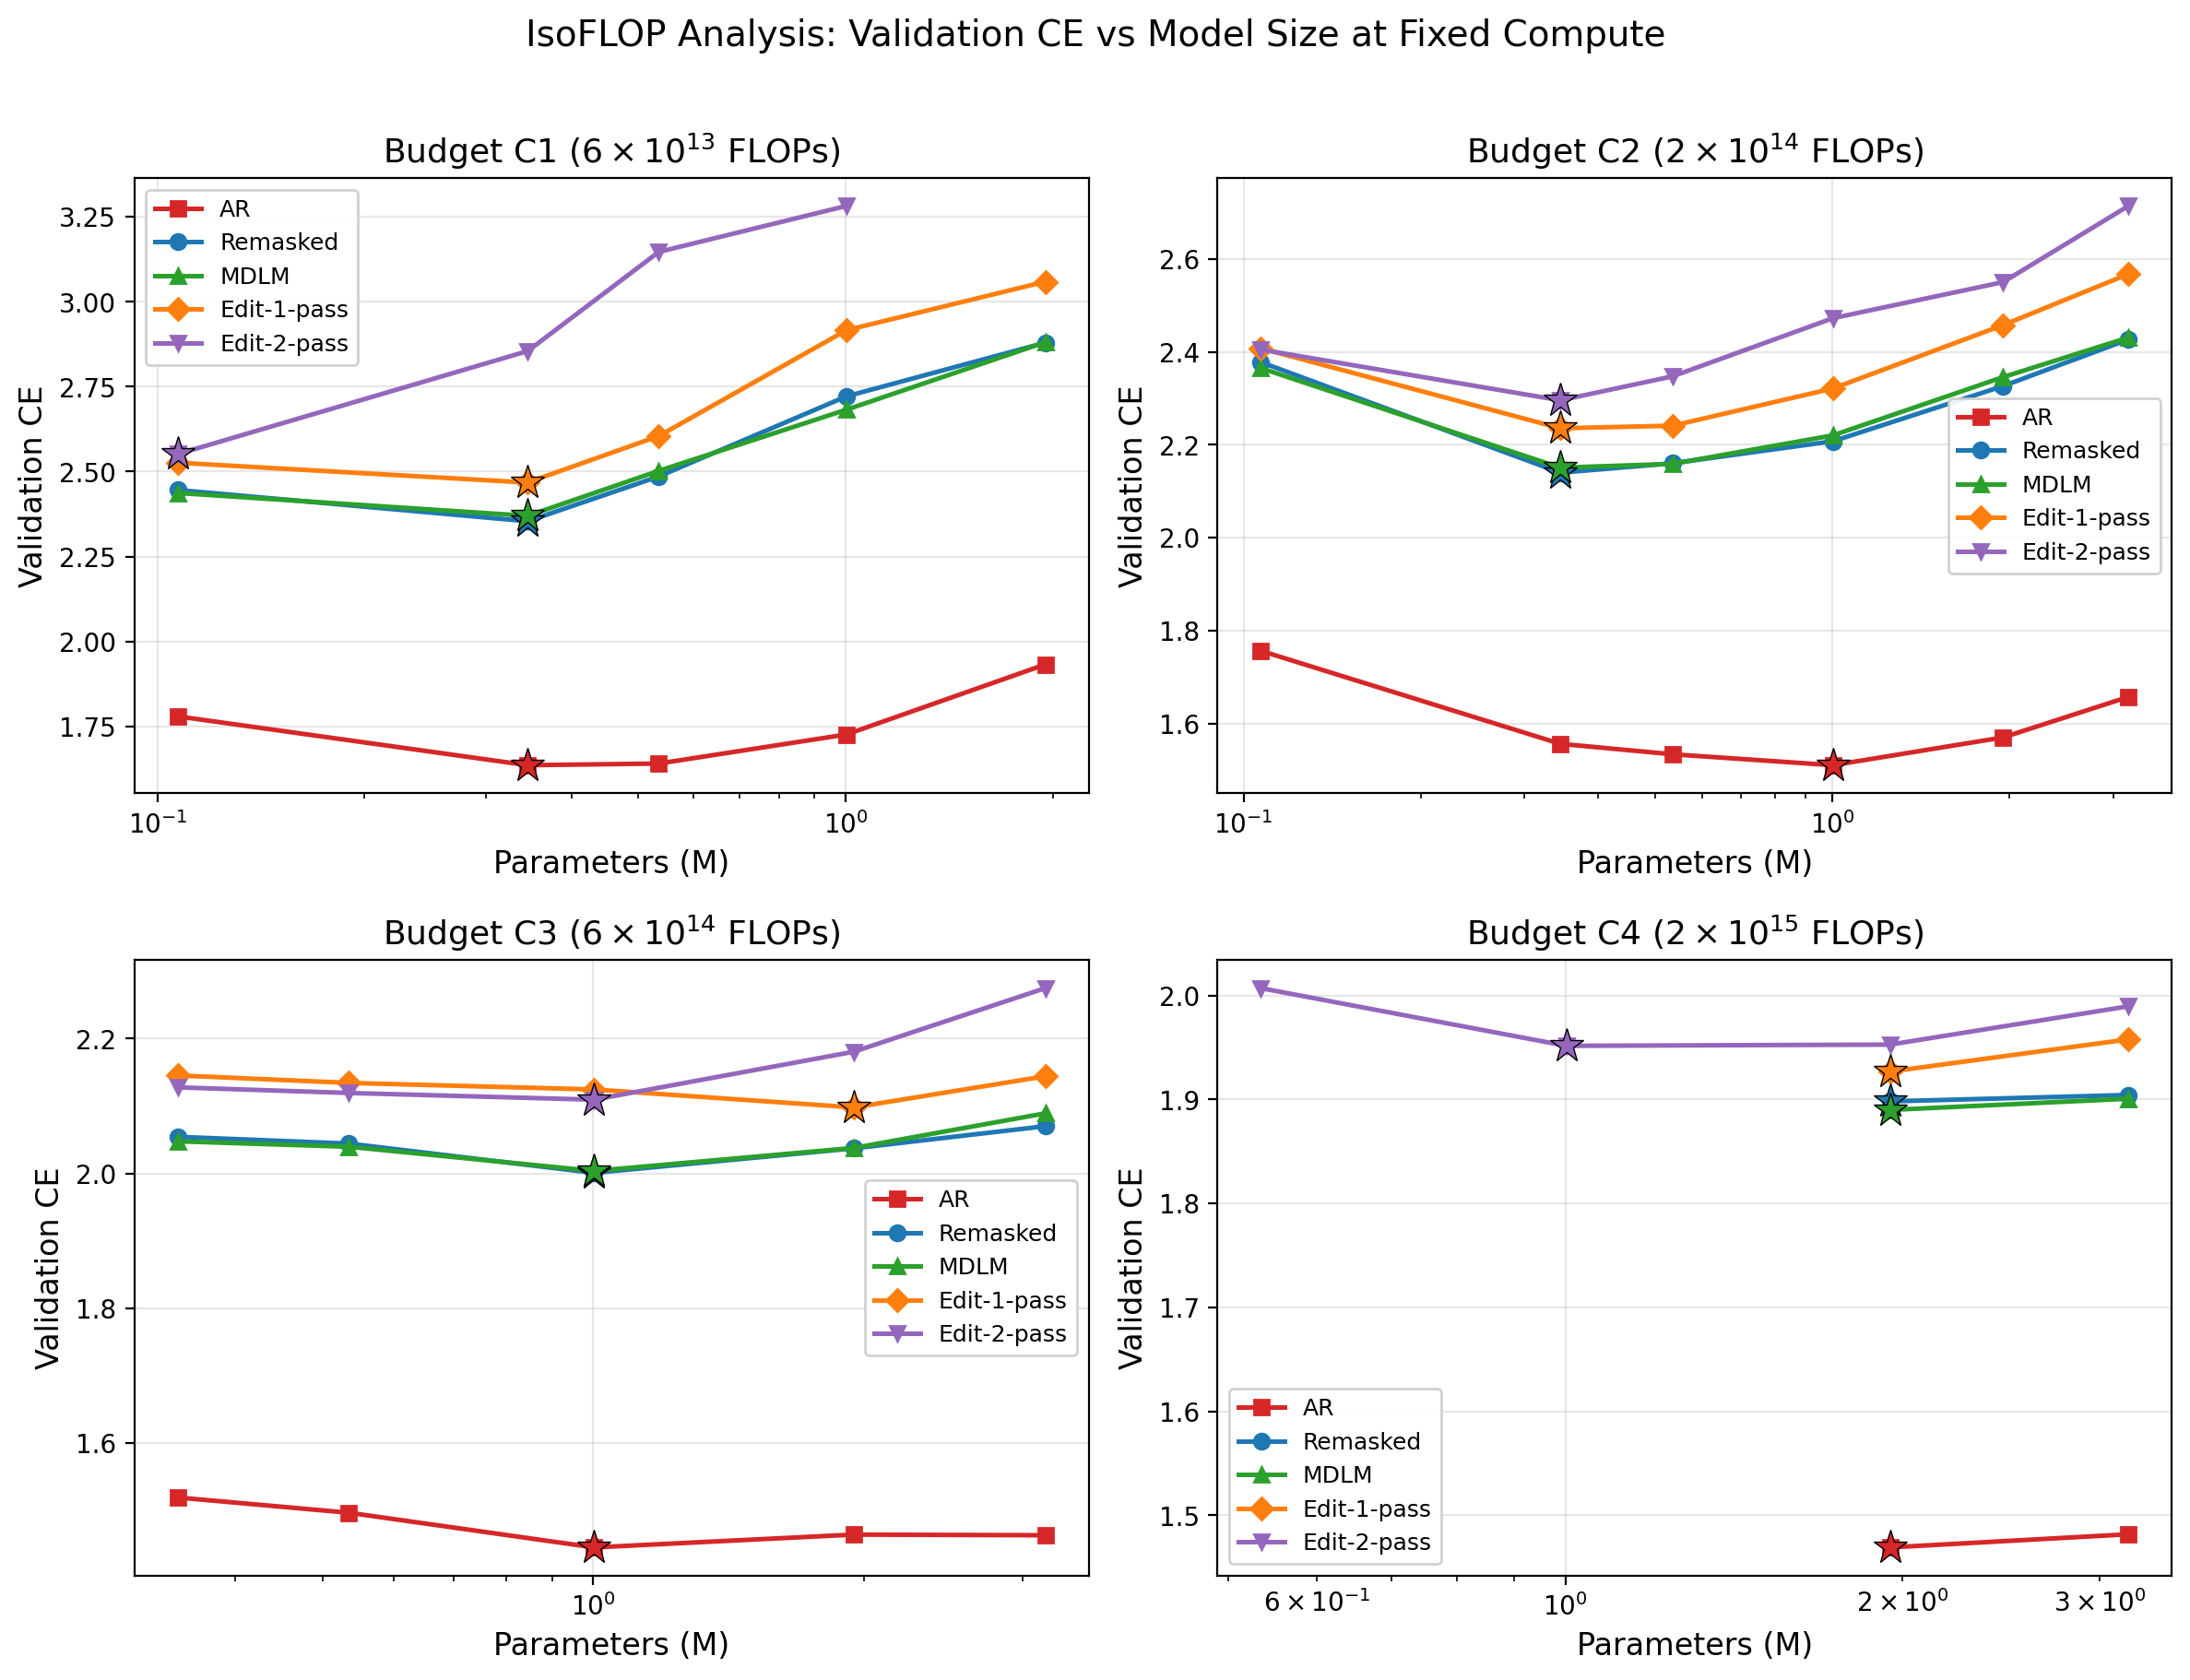
\includegraphics[width=\textwidth]{isoflop/isoflop_curves.png}
    \caption{IsoFLOP curves across four FLOP budgets. Stars mark the lowest validation CE within each family. The main signal is how those stars move as the budget increases.}
    \label{fig:isoflop-curves}
\end{figure}

At C1, the minima are similar: 0.3M for AR, Remasked, MDLM, and Edit-one-pass; 0.1M for the more expensive Edit-two-pass.
The family split appears at C2.
AR now prefers 1M, while Remasked, MDLM, and Edit-one-pass still prefer 0.3M.
This is the clearest budget in the study because the search space is fully covered and the minimum is not yet distorted by the 10k-step cap.

\subsection{AR Moves to Larger Models Earlier Than Diffusion}

Figure~\ref{fig:frontier} summarizes the main pattern.
The right panel tracks the compute-optimal model size as the budget grows.
AR leaves the 0.3M regime at the second budget.
Remasked and MDLM do not do so until the third.
Edit-one-pass is intermediate: it stays at 0.3M through C2, then jumps more aggressively at C3.

\begin{figure}[H]
    \centering
    \begin{subfigure}[t]{0.48\textwidth}
        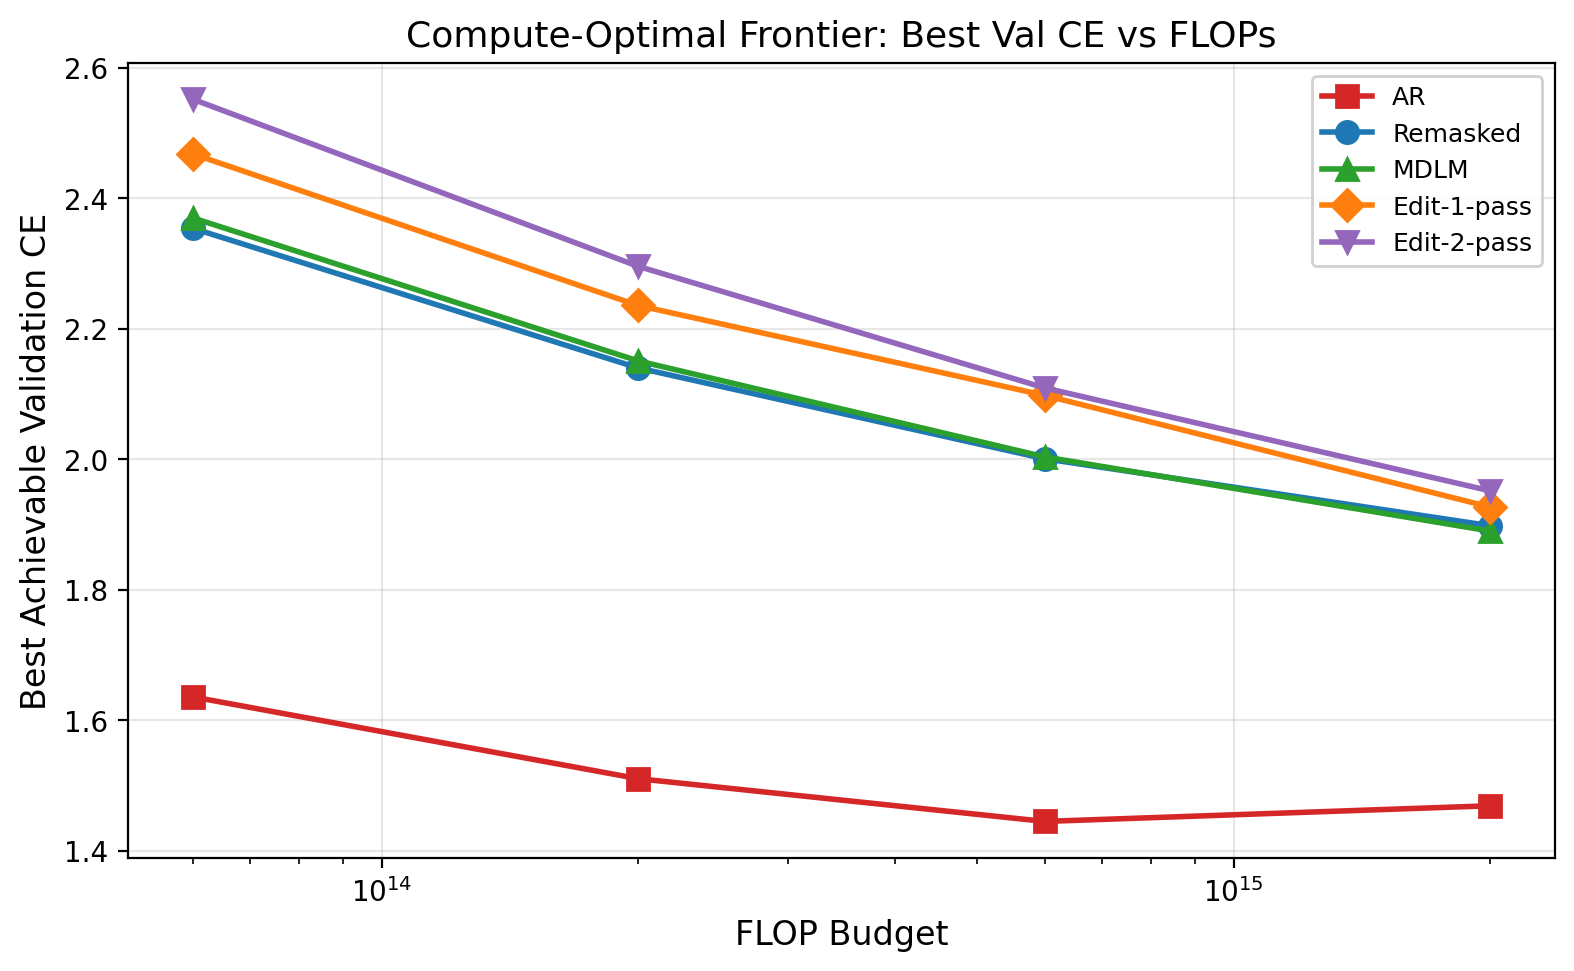
\includegraphics[width=\textwidth]{isoflop/compute_optimal_frontier.png}
        \caption{Best validation CE within each family at each budget.}
        \label{fig:frontier-val}
    \end{subfigure}
    \hfill
    \begin{subfigure}[t]{0.48\textwidth}
        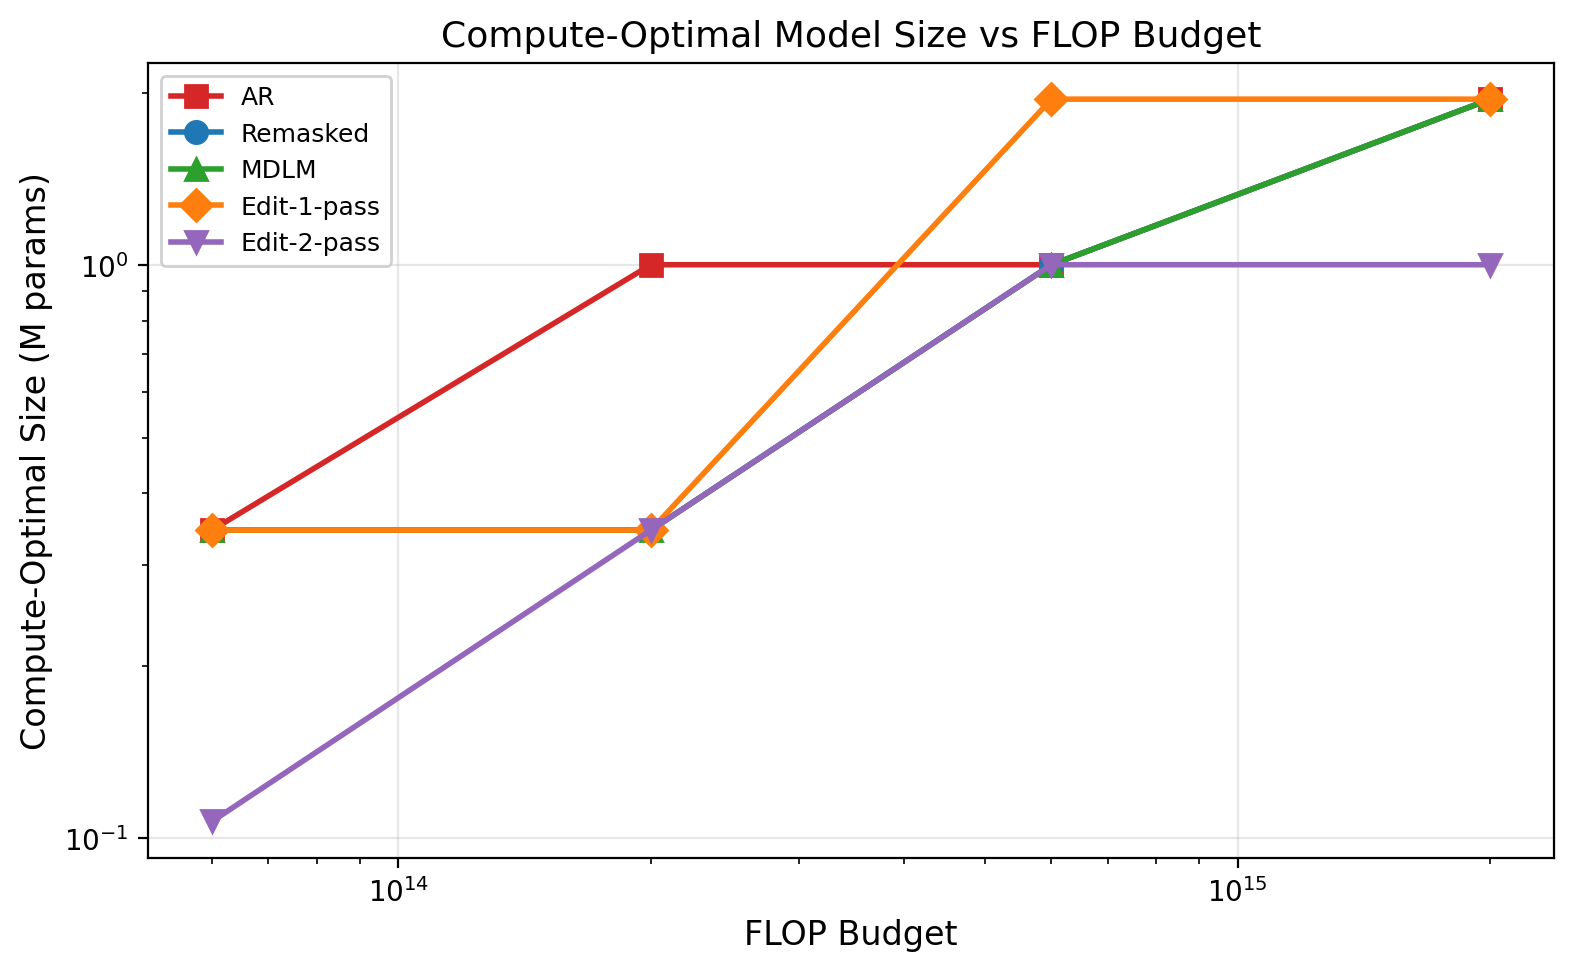
\includegraphics[width=\textwidth]{isoflop/optimal_size_vs_budget.png}
        \caption{Compute-optimal size vs.\ FLOP budget.}
        \label{fig:frontier-size}
    \end{subfigure}
    \caption{Left: best validation CE within each family. Right: the compute-optimal size path. The most important comparison is not absolute CE across families, but when each family decides it is worth paying for a larger model.}
    \label{fig:frontier}
\end{figure}

The cleanest intuition comes from C2.
Under the same FLOP budget, AR prefers a 1M model trained for 1015 steps.
Remasked and MDLM prefer a 0.3M model trained for 2948 steps.
That is not a small numerical shift; it is a different compute-allocation strategy.
AR spends the new budget on parameters earlier.
Diffusion spends it on updates.
At higher budgets the minima also become fairly broad, especially near C4.
So the robust claim is the direction of movement, not that, say, 2M is decisively better than 3M at the top budget.

\subsection{Overfitting Explains Most of the Difference}

Figure~\ref{fig:isoflop-gap} gives the likely reason.
At each budget, we plot the overfitting gap, defined as validation CE minus training CE.
The gap grows for every family as compute increases, but it grows much faster for AR.

\begin{figure}[H]
    \centering
    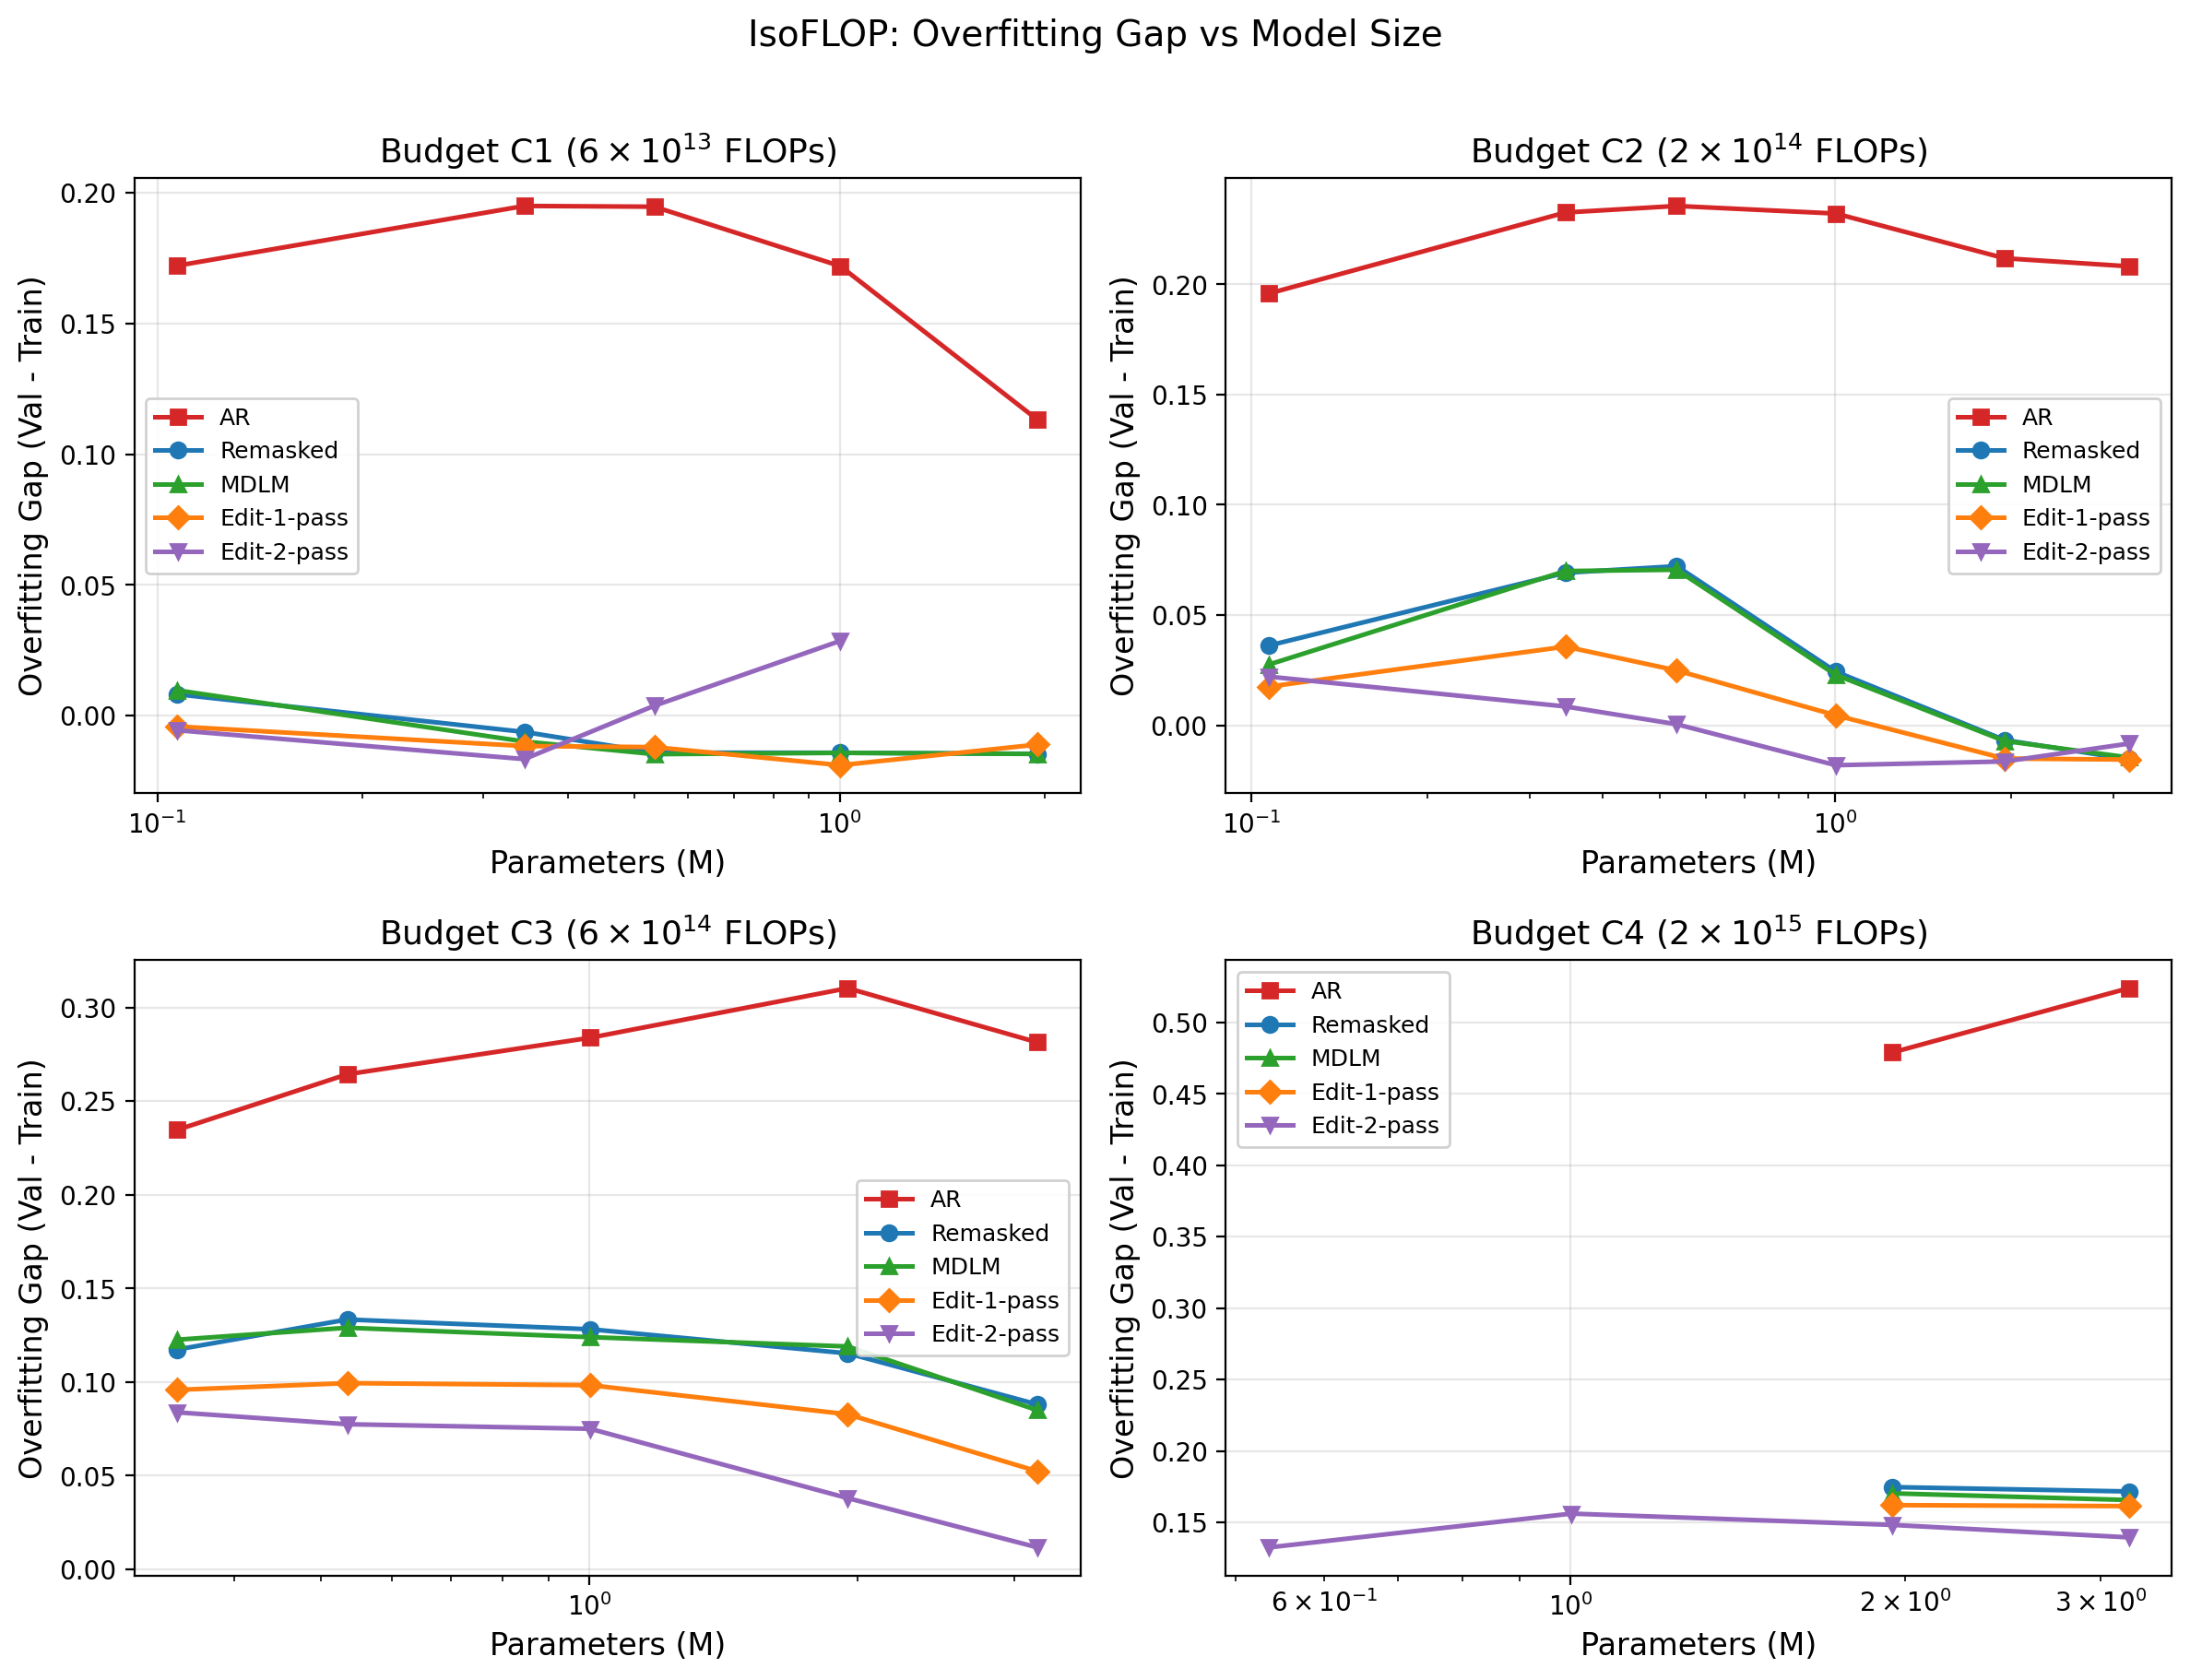
\includegraphics[width=\textwidth]{isoflop/isoflop_gap.png}
    \caption{Overfitting gap in the IsoFLOP regime. AR's gap rises sharply with budget. The diffusion families remain much more controlled and are slightly underfit at the smallest budget.}
    \label{fig:isoflop-gap}
\end{figure}

At the compute-optimal point, AR's gap grows from 0.195 at C1 to 0.479 at C4.
The diffusion families stay below 0.18 throughout, and several of them have slightly negative gaps at C1.
That negative gap is useful intuition: at low budget, the denoising objective is noisy enough that the model is not even fully fitting the training set.
In other words, diffusion starts from an underfitting problem, while AR starts much closer to a memorization problem.

This difference naturally changes how extra compute should be spent.
If longer training mostly pushes AR deeper into memorization, then scaling up becomes attractive earlier.
If longer training remains productive for diffusion, then staying smaller for longer is reasonable.
That is the sense in which masking noise acts like built-in regularization.

One consequence shows up in the left panel of Figure~\ref{fig:frontier}.
The best AR run improves from C1 to C3, then slightly worsens at C4.
That is consistent with a dataset bottleneck: more compute is available, but it is no longer easy to turn that compute into better validation loss.

\subsection{Within the Diffusion Family, the Differences Are Smaller}

The diffusion variants do not separate dramatically.
Remasked and MDLM are nearly identical at every budget, which is plausible because they share the same denoising objective and mostly differ at inference time.
Edit-one-pass trails them slightly but follows the same broad scaling pattern.

Edit-two-pass is the most distinct case.
Because each step is twice as expensive, it tends to prefer smaller models.
Even so, it does not collapse.
At C4 its best validation CE (1.952) is close to Edit-one-pass (1.927), suggesting that the correction pass recovers some of the value lost to the reduced update count.

\subsection{Summary Table}

\begin{table}[H]
\centering
\caption{Compute-optimal configuration within each family and budget. The main columns to watch are optimal size and overfitting gap.}
\label{tab:isoflop-optimal}
\begin{tabular}{llrrrr}
\toprule
Budget & Model & Opt.\ Size & Val CE & Train CE & Gap \\
\midrule
\multirow{5}{*}{C1 ($6\!\times\!10^{13}$)} & AR & 0.3M & 1.636 & 1.441 & 0.195 \\
& Remasked & 0.3M & 2.354 & 2.360 & $-$0.006 \\
& MDLM & 0.3M & 2.370 & 2.380 & $-$0.010 \\
& Edit-1-pass & 0.3M & 2.468 & 2.480 & $-$0.012 \\
& Edit-2-pass & 0.1M & 2.552 & 2.557 & $-$0.006 \\
\midrule
\multirow{5}{*}{C2 ($2\!\times\!10^{14}$)} & AR & 1M & 1.511 & 1.278 & 0.232 \\
& Remasked & 0.3M & 2.140 & 2.071 & 0.069 \\
& MDLM & 0.3M & 2.151 & 2.081 & 0.070 \\
& Edit-1-pass & 0.3M & 2.236 & 2.200 & 0.036 \\
& Edit-2-pass & 0.3M & 2.296 & 2.287 & 0.009 \\
\midrule
\multirow{5}{*}{C3 ($6\!\times\!10^{14}$)} & AR & 1M & 1.445 & 1.161 & 0.284 \\
& Remasked & 1M & 2.001 & 1.873 & 0.128 \\
& MDLM & 1M & 2.004 & 1.880 & 0.124 \\
& Edit-1-pass & 2M & 2.098 & 2.015 & 0.083 \\
& Edit-2-pass & 1M & 2.109 & 2.034 & 0.075 \\
\midrule
\multirow{5}{*}{C4 ($2\!\times\!10^{15}$)} & AR & 2M & 1.469 & 0.990 & 0.479 \\
& Remasked & 2M & 1.898 & 1.723 & 0.175 \\
& MDLM & 2M & 1.890 & 1.720 & 0.170 \\
& Edit-1-pass & 2M & 1.927 & 1.765 & 0.162 \\
& Edit-2-pass & 1M & 1.952 & 1.795 & 0.156 \\
\bottomrule
\end{tabular}
\end{table}

%% ===================================================================
\section{Takeaways and Limits}
\label{sec:discussion}

\paragraph{What the paper shows.}
In this small-data setting, objective choice changes the compute-optimal scaling path.
AR moves to larger models earlier.
Diffusion stays smaller for longer and spends more of the budget on updates.
The overfitting-gap plots make that pattern intelligible rather than mysterious.

\paragraph{What the paper does not show.}
It does not show that diffusion is better than AR in an absolute sense.
Cross-family validation CE is not directly comparable, and this dataset is intentionally chosen to make overfitting visible.
It also does not show what happens once the data bottleneck weakens.
On a much larger corpus, AR may not hit the same wall.

\paragraph{How to read the practical implication.}
The practical takeaway is narrow but useful.
If data is scarce relative to capacity, then the denoising objective appears to buy regularization ``for free,'' and that changes how compute should be allocated.
The result is less ``train diffusion because it wins'' and more ``expect a different scaling law when the objective injects noise throughout training.''

\paragraph{Next steps.}
The most useful follow-up is not more rhetoric on TinyShakespeare but a larger-scale replication with a shared downstream metric.
That means a larger corpus, subword tokenization, multiple random seeds, and an evaluation that is comparable across paradigms.
The IsoFLOP machinery here is still useful; it just needs a setting where the top budget is not truncated by a step cap and where cross-family quality can be measured directly.

%% ===================================================================
\begin{appendices}

\section{Hyperparameter Sweep}
\label{app:sweep}

We swept learning rate $\in \{3\!\times\!10^{-4},\;10^{-3},\;3\!\times\!10^{-3},\;10^{-2}\}$ and batch size $\in \{64, 128\}$ for each (model, size) pair at 800 training steps.
Batch size 128 was consistently preferred.
Table~\ref{tab:optimal-lr} shows the optimal learning rates.

\begin{table}[H]
\centering
\caption{Optimal learning rate from 800-step sweep. All at batch size 128.}
\label{tab:optimal-lr}
\begin{tabular}{lcccc}
\toprule
Model & 0.1M & 0.3M & 1M & 3M \\
\midrule
Remasked     & $10^{-2}$ & $3\!\times\!10^{-3}$ & $3\!\times\!10^{-3}$ & $3\!\times\!10^{-3}$ \\
MDLM         & $10^{-2}$ & $3\!\times\!10^{-3}$ & $3\!\times\!10^{-3}$ & $3\!\times\!10^{-3}$ \\
Edit-one-pass & $10^{-2}$ & $10^{-2}$ & $10^{-2}$ & $3\!\times\!10^{-3}$ \\
Edit-two-pass & $10^{-2}$ & $3\!\times\!10^{-3}$ & $3\!\times\!10^{-3}$ & $3\!\times\!10^{-3}$ \\
AR           & $10^{-2}$ & $10^{-2}$ & $10^{-2}$ & $3\!\times\!10^{-3}$ \\
\bottomrule
\end{tabular}
\end{table}

\section{Fixed-Step Scaling (Dropout = 0.1)}
\label{app:scaling}

Before the IsoFLOP experiments, we ran all families at 4000 fixed training steps with dropout\,=\,0.1 to establish baseline scaling behavior.
The key observation: the AR 3M model catastrophically overfits (gap\,=\,1.018), while all diffusion families scale smoothly with gaps $<$\,0.2.

\begin{figure}[H]
    \centering
    \begin{subfigure}[t]{0.48\textwidth}
        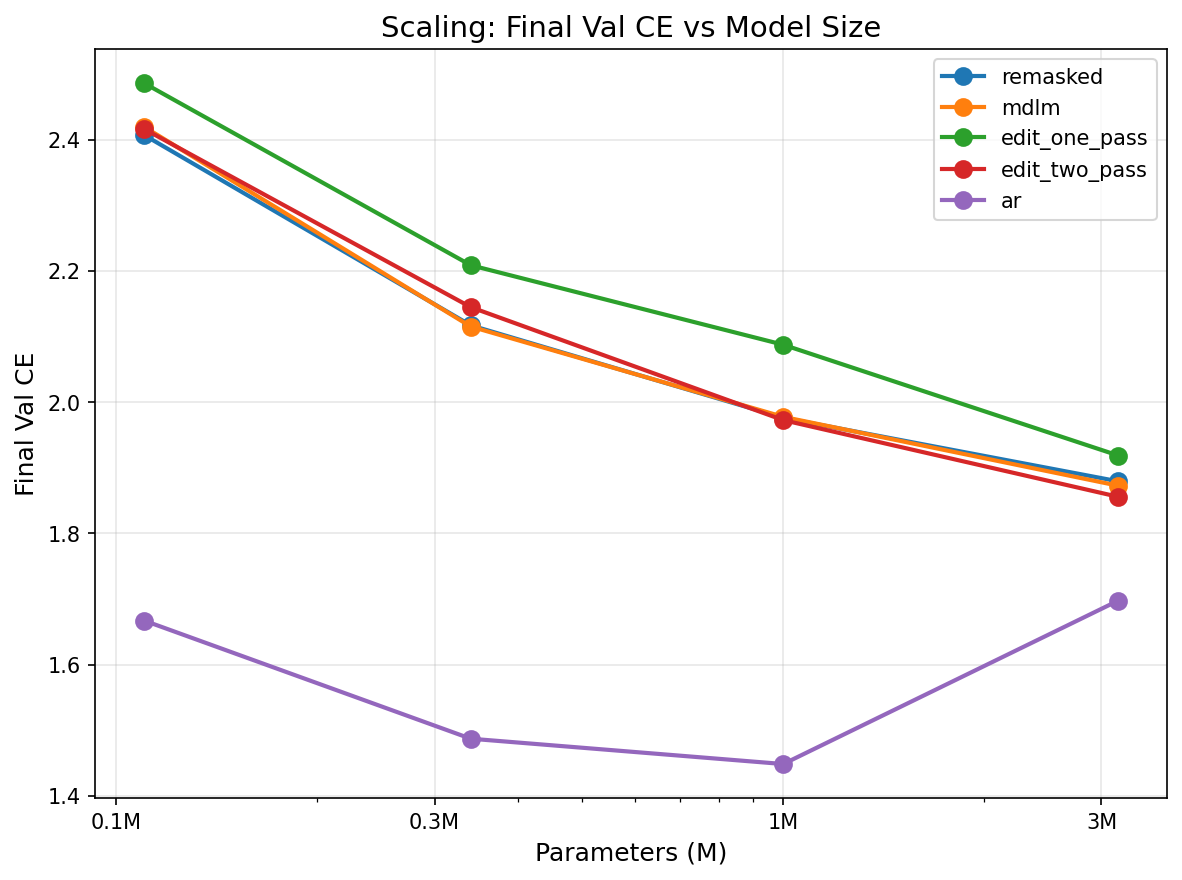
\includegraphics[width=\textwidth]{scaling/scaling_val_ce.png}
        \caption{Final validation CE vs.\ model size.}
    \end{subfigure}
    \hfill
    \begin{subfigure}[t]{0.48\textwidth}
        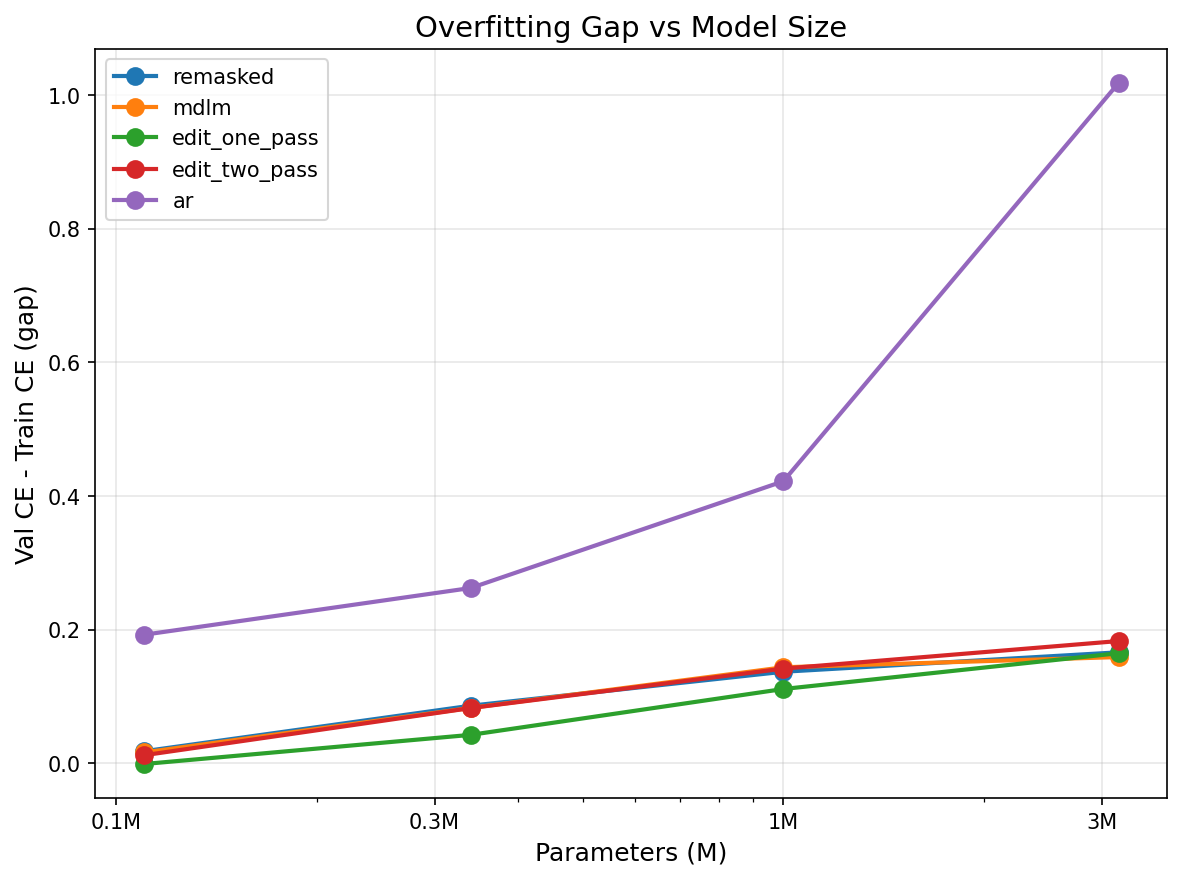
\includegraphics[width=\textwidth]{scaling/overfitting_gap.png}
        \caption{Overfitting gap.}
    \end{subfigure}
    \caption{Scaling at dropout\,=\,0.1. AR degrades at 3M due to catastrophic overfitting (gap $>$ 1.0). Diffusion models scale smoothly.}
    \label{fig:scaling-01}
\end{figure}

\begin{table}[H]
\centering
\caption{Full scaling results at dropout\,=\,0.1, 4000 steps. AR 3M highlighted.}
\label{tab:scaling-01}
\begin{tabular}{llrrr}
\toprule
Model & Size & Train CE & Val CE & Gap \\
\midrule
Remasked     & 0.1M & 2.389 & 2.407 & 0.018 \\
             & 0.3M & 2.031 & 2.117 & 0.086 \\
             & 1M   & 1.839 & 1.976 & 0.137 \\
             & 3M   & 1.713 & 1.879 & 0.166 \\
\midrule
MDLM         & 0.1M & 2.403 & 2.420 & 0.016 \\
             & 0.3M & 2.032 & 2.115 & 0.083 \\
             & 1M   & 1.834 & 1.978 & 0.144 \\
             & 3M   & 1.713 & 1.873 & 0.159 \\
\midrule
Edit-one-pass & 0.1M & 2.487 & 2.486 & $-$0.001 \\
              & 0.3M & 2.166 & 2.209 & 0.043 \\
              & 1M   & 1.976 & 2.087 & 0.111 \\
              & 3M   & 1.754 & 1.919 & 0.165 \\
\midrule
Edit-two-pass & 0.1M & 2.404 & 2.416 & 0.012 \\
              & 0.3M & 2.062 & 2.145 & 0.083 \\
              & 1M   & 1.831 & 1.973 & 0.142 \\
              & 3M   & 1.673 & 1.856 & 0.183 \\
\midrule
AR            & 0.1M & 1.475 & 1.667 & 0.193 \\
              & 0.3M & 1.225 & 1.487 & 0.263 \\
              & 1M   & 1.026 & 1.449 & 0.422 \\
              & \textbf{3M}   & \textbf{0.679} & \textbf{1.698} & \textbf{1.018} \\
\bottomrule
\end{tabular}
\end{table}

\begin{figure}[H]
    \centering
    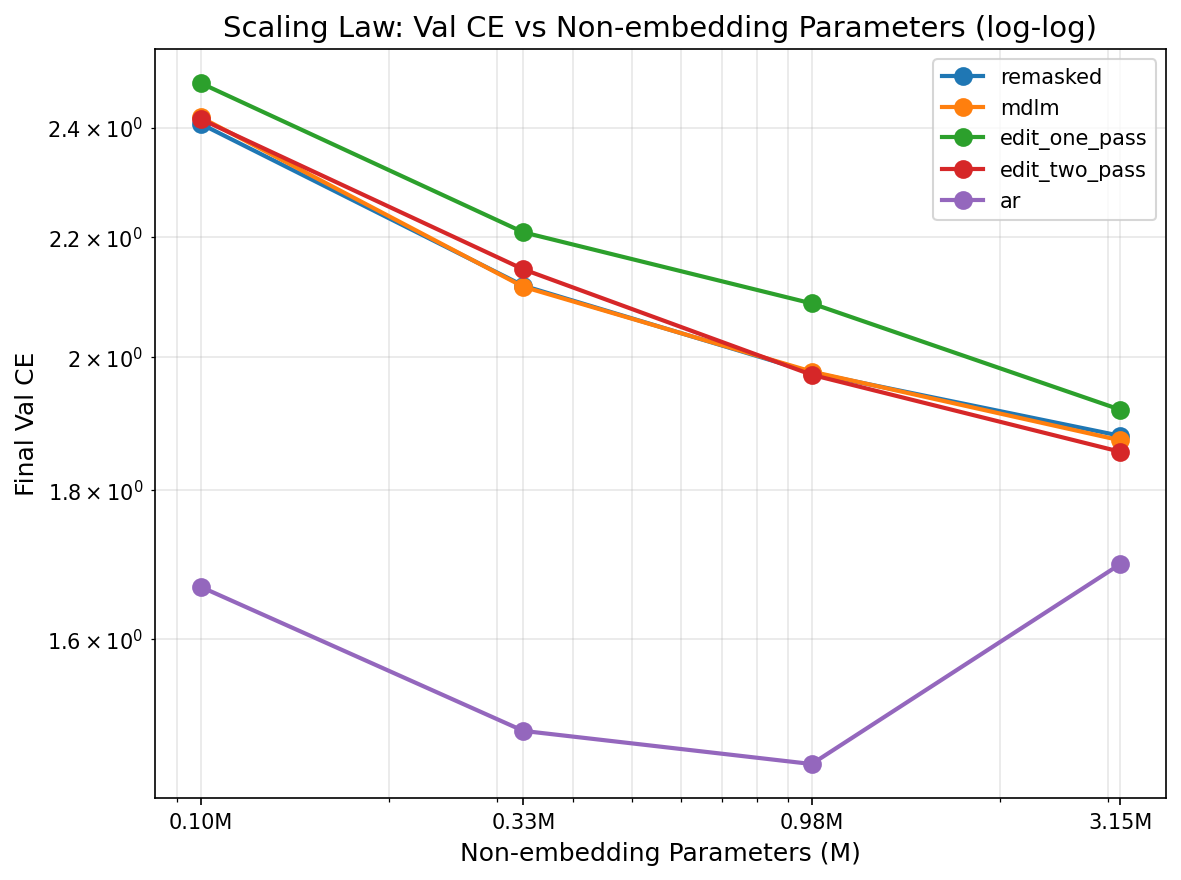
\includegraphics[width=0.6\textwidth]{scaling/scaling_loglog.png}
    \caption{Log-log scaling. Diffusion models follow clean power laws; AR deviates at 3M.}
    \label{fig:loglog}
\end{figure}

\section{Why Extra Dropout Hurts Diffusion Models}
\label{app:dropout}

We reran all configurations with dropout\,=\,0.2.
For AR at 3M, this dramatically helps: val CE drops from 1.698 to 1.493, and the gap shrinks from 1.018 to 0.574.
For \emph{every} diffusion family, dropout\,=\,0.2 uniformly \emph{hurts}, degrading val CE by 0.04--0.18.

\begin{figure}[H]
    \centering
    \begin{subfigure}[t]{0.48\textwidth}
        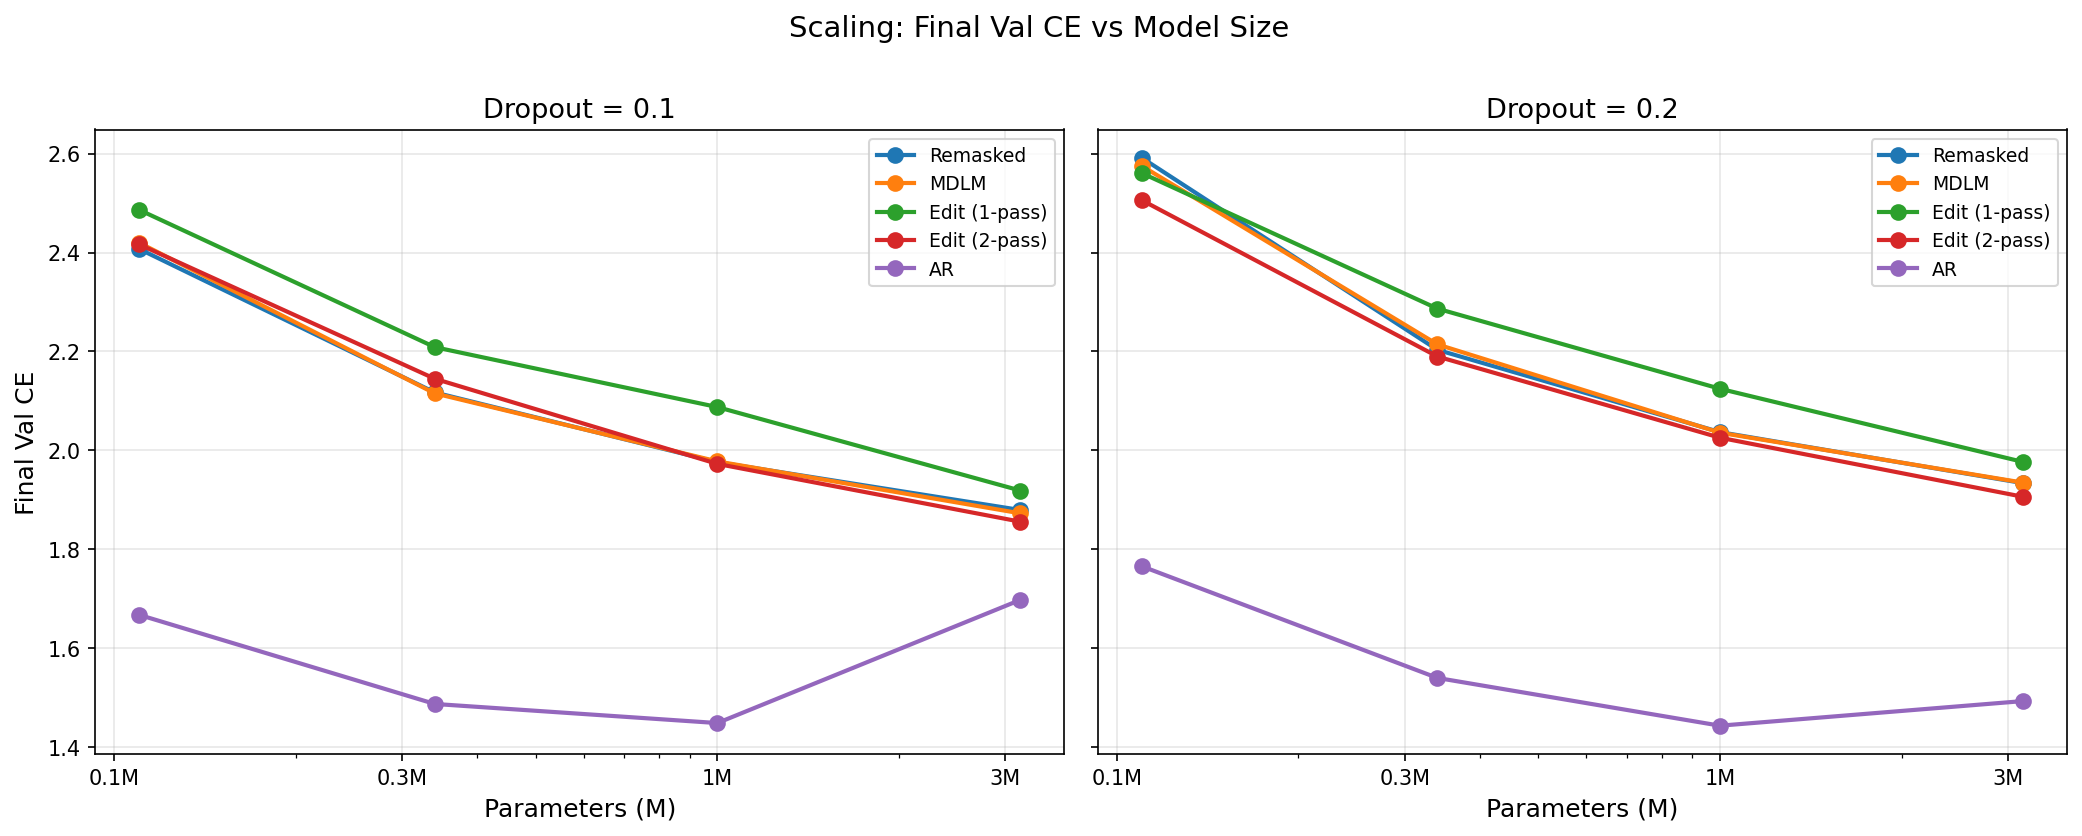
\includegraphics[width=\textwidth]{scaling_comparison_val_ce.png}
        \caption{Validation CE: dropout 0.1 vs.\ 0.2.}
    \end{subfigure}
    \hfill
    \begin{subfigure}[t]{0.48\textwidth}
        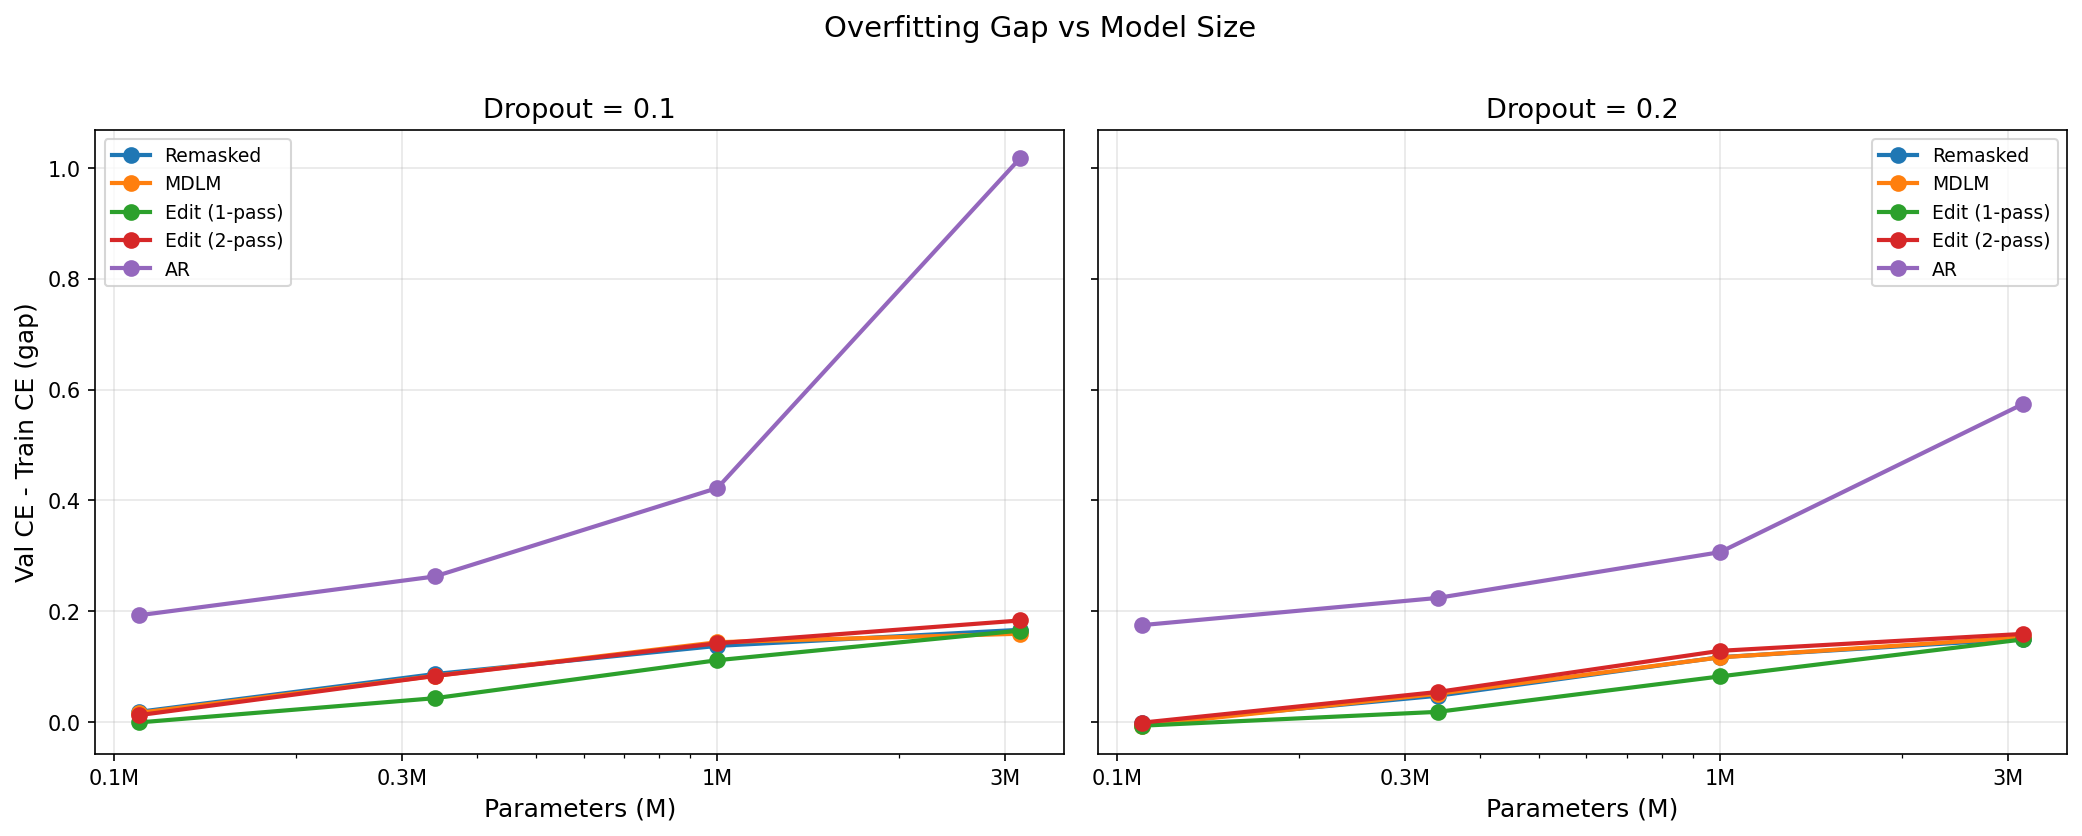
\includegraphics[width=\textwidth]{scaling_comparison_gap.png}
        \caption{Overfitting gap: dropout 0.1 vs.\ 0.2.}
    \end{subfigure}
    \caption{Dropout comparison. AR benefits from more dropout at 3M; diffusion models are harmed at every size.}
    \label{fig:dropout-comparison}
\end{figure}

The interpretation is straightforward: masking noise during diffusion training already provides strong regularization.
Adding dropout on top is \emph{redundant}---it doesn't reduce overfitting (which is already minimal) but does reduce effective model capacity.
This is why all IsoFLOP experiments use dropout\,=\,0.1 for diffusion and dropout\,=\,0.2 for AR.

\begin{figure}[H]
    \centering
    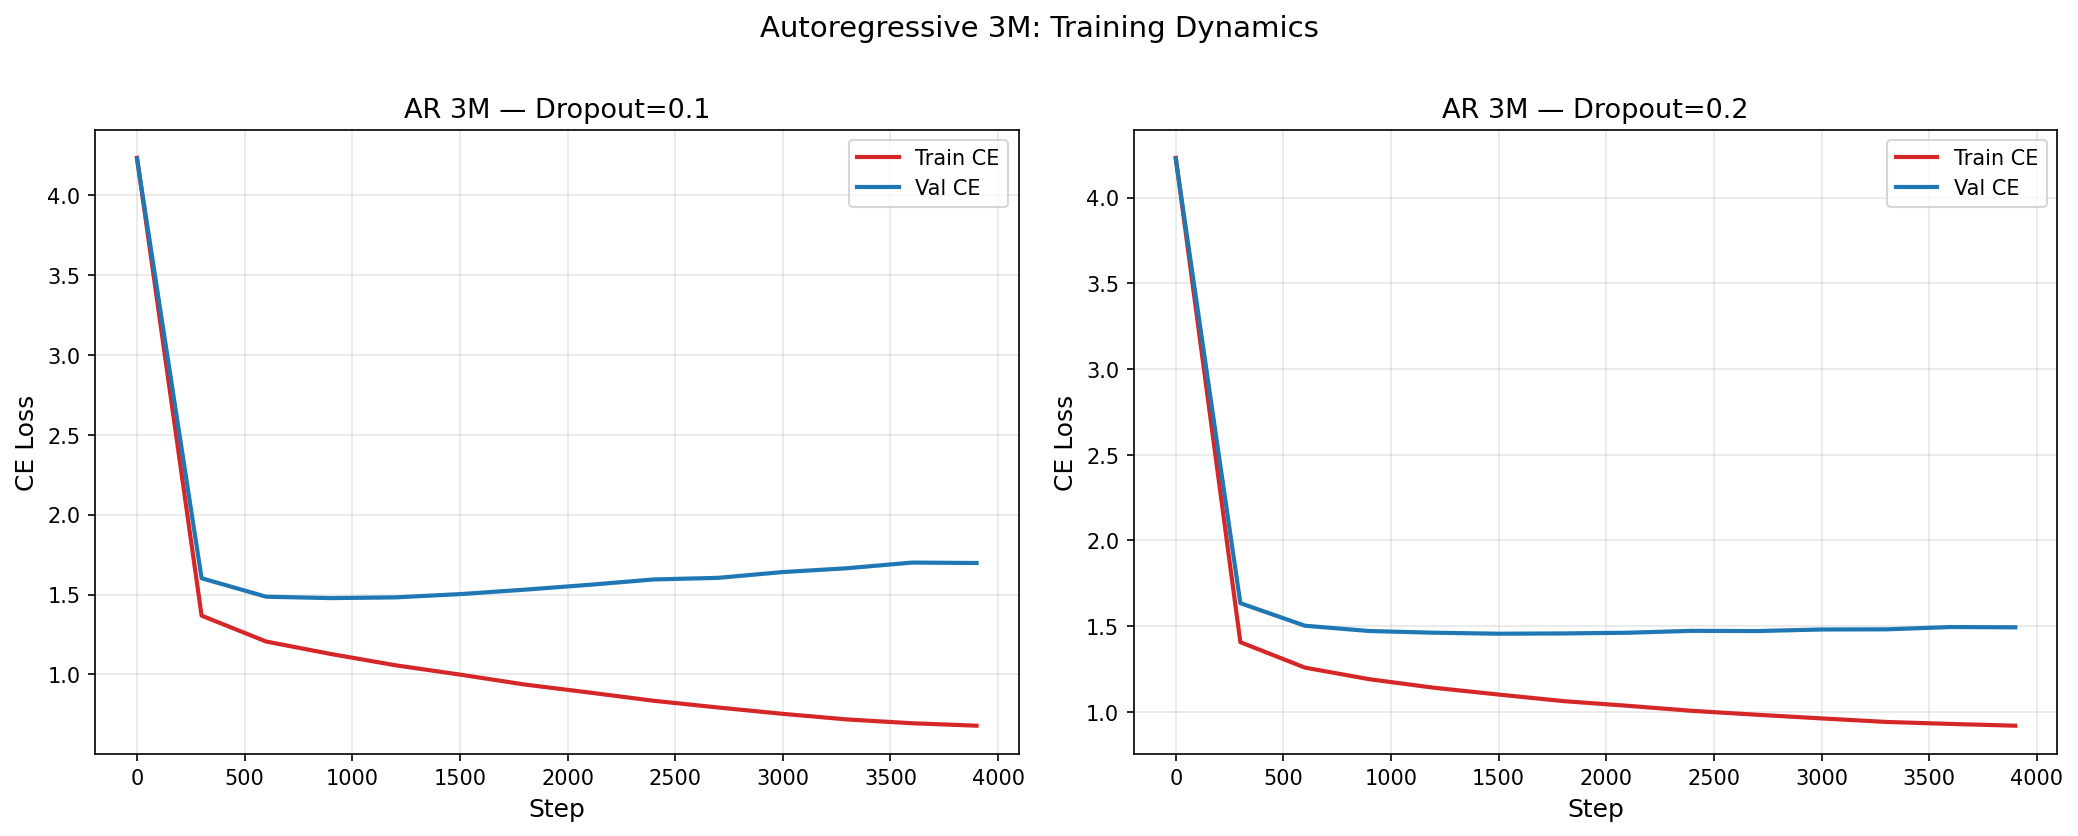
\includegraphics[width=0.85\textwidth]{ar_3m_dynamics.png}
    \caption{AR 3M training dynamics. Left (dropout\,=\,0.1): val CE rises after step ${\sim}500$---the model is memorizing. Right (dropout\,=\,0.2): memorization is suppressed, but the gap is still 0.574.}
    \label{fig:ar-dynamics}
\end{figure}

\end{appendices}

\end{document}
